
\documentclass[11pt]{article}
\usepackage{amsmath}
\usepackage{siunitx}
\usepackage{graphicx, float}
\usepackage[plain]{algorithm}

\topmargin=-0.45in
\evensidemargin=0in
\oddsidemargin=0in
\textwidth=6.5in
\textheight=9.0in
\headsep=0.25in


\title{Measuring Modes on Strings: Part 1}
\author{Alex Booth}

\bibliographystyle{plain}



\begin{document}
    \maketitle

    \section{Introduction}
        This report details an investigation into the phenomena observed on a vibrating string.
        Several experiments took place, using a guitar, as guitars feature strings under tension that can freely vibrate.
        The frequency and amplitude of vibrations can be easily and precisely adjusted on a well-intonated guitar by fretting the strings along the fingerboard.
        Results are tabulated and plotted on graphs using MATLAB. 
    
    \section{Theory}
        Strings held under tension by two boundary conditions can facilitate standing waves.
        A standing wave is a wave travelling through a medium, in this case the string, oscillating in time.
        However, due to the distance between the boundary conditions being an integer multiple of the incident wavelength, after reflecting when reaching the boundary conditions of the medium, it appears to not oscillate in time, due to the constructive or destructive interference of the incident and reflected wave \cite{STWAVES20, PHYS15}.
        A string vibrates with a fundamental, or in music theory tonic, frequency.
        This fundamental frequency is related to the length $L$ of a vibrating string:
        \begin{equation}
            f_1 = \frac{c}{2 L}
        \end{equation}
        The mass of a string and its length can be used to find a mass per unit length $M$.
        This mass per unit length can then be formulated with it's tension $T$ to find the speed of a transverse wave on a string:
        \begin{equation}\label{speed}
            c = \sqrt{\frac{T}{M}}
        \end{equation}
        Equation \ref{speed} allows us to formulate:
        \begin{equation}\label{fund}
            f_1 = \frac{\sqrt{\frac{T}{M}}}{2 L}
        \end{equation}
        If the ends of a string under tension are fixed, the fundamental frequency will have a wavelength equal to half the string's length.
        The frequencies of higher harmonics of the fundamental frequency are integer multiples of the fundamental frequency:
        \begin{equation}\label{harm}
            f_n = \frac{c}{2 L} n
        \end{equation}

    \section{Experiment One}
        \subsection{Methodology and Results}
            In experiment one, the relationship between resonant frequency and string length were investigated.
            Preliminary measurements of mass and length were taken in order to find a mass per unit length $M = 0.012618\si{\kilogram\per\meter}$.
            Then the low E string was played in an open position, thus at it's maximum string length and at a frequency of $83\si{\hertz}$.
            Using equation \ref{harm} the higher harmonics $n = 1, 2 ,3 ...$ are predicted for the vibrating open E string.
            The sound of the vibrating string was captured using a microphone and passed into a Simulink frequency spectrum analyser.
            From this spectrum analyser the frequencies of the fundamental tone and it's higher harmonics could be ascertained.
            However, not every frequency in the harmonic series had a sufficient amplitude to be declared a peak by the Simulink spectrometer, meaning that the recorded harmonic series will have gaps compared to the array of predicted harmonic frequencies.
            Rearranging equation \ref{harm} allowed a wave speed $c_n$ to be found for each harmonic number, for both the predicted and recorded harmonics.
            To compare the error between the predicted and observed harmonic wave speeds, a mean wave speed was taken for the observed values.
            The difference between this mean wave speed $c$ and each predicted harmonic wave speed $c_n$ was then taken.
            These differences were then summed and divided by the number of harmonics to give a mean difference and thus average error:
            \begin{equation}
                \Delta c = \frac{1}{N}\sum_{n=1}^{N} | c_n - c |
            \end{equation}
            The array of predicted wave speeds for harmonic numbers up to harmonic number $n=6$ are tabulated:
            \begin{table}[H]
                \centering
                \begin{tabular}{c | l l l l l l}
                    \hline
                    $n$ & 1 & 2 & 3 & 4 & 5 & 6 \\
                    \hline
                    $c(\si{\meter\per\second})$ & 102.7 & 205.41 & 308.12 & 410.83 & 513.54 & 616.24 \\
                    \hline
                \end{tabular}
                \caption{Predicted wave speeds for each harmonic}
            \end{table}
            The average error $\Delta c$ was calculated: $\Delta c = 3.4$.
            Next, the guitar string was plucked whilst fretted on the fingerboard.
            The fundamental frequency for the fretted note (A - the 5\textsuperscript{th} fret on the E string) was predicted to be $f=110\si{\hertz}$ using equations \ref{speed} and \ref{harm}.
            The recorded frequency was found to be $f=112\si{\hertz}$.
            The string was fretted at a series of frets and the fundamental frequencies were tabulated:
            \begin{table}[H]
                \centering
                \begin{tabular}{c | l l l l}
                    \hline
                    Fret & 0 & 3 & 5 & 12 \\
                    \hline
                    Distance from bridge (\si{\meter}) & 0.645 & 0.534 & 0.477 & 0.318 \\
                    \hline
                    $f_1(\si{\hertz})$ & 81 & 97 & 113 & 167 \\
                    \hline
                \end{tabular}
                \caption{Fundamental frequencies of each fretted note}
            \end{table}
            Using equation \ref{fund}, an array of predicted values for fundamental frequency can be found and plotted against string length.
            The observed fundamental frequencies for each fretted note are also plotted on the same graph.
            \begin{figure}[H]\label{f1vsl}
                \centering
                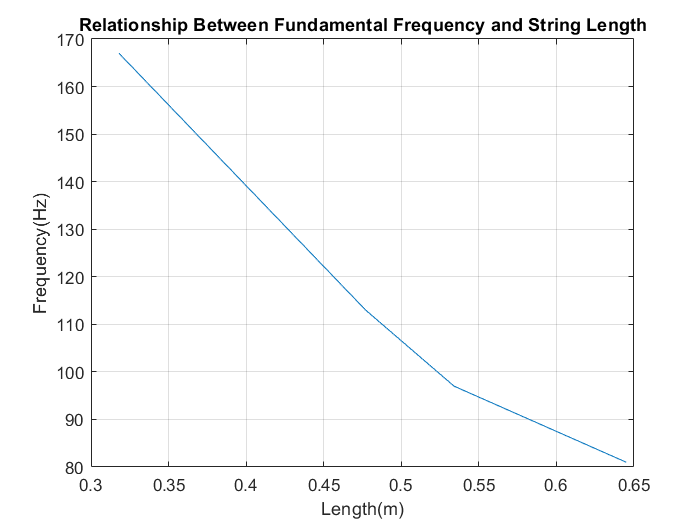
\includegraphics[scale=0.5]{resources/F1vsL.png}
                \caption{Predicted and measured frequency dependence on string length}
            \end{figure}
        \subsection{Discussion of Results}
            Such a high error in $c$ can be attributed to the missing harmonic frequencies from the observed series, and the frequency response of the microphone used to capture the sound "colouring" the signal.
            In Fig.\ref{f1vsl} the predicted and measured frequency dependence on string length follow each other closely, adopting a similar pattern.
            The resolution of the measured results was much lower than the predicted results, and this is clearly visible on the graph.
            This resolution can be improved by collecting a larger data set, by recording the fundamental frequency of every fret along the fingerboard.
            
    \section{Experiment 2}
        Rearranging equation \ref{speed} allows us to find a value of Tension $T$ for the open string.
        The error of the results $\Delta T$ is depended on the error $\Delta c$. And thus the error $\Delta T$ was calculated:
        \begin{align}
            \frac{\Delta T}{T} & = 2 \frac{\Delta c}{c}\\
            \Delta T & = 2 T \frac{\Delta c}{c} = 5.88
        \end{align}
        Rearranging equations \ref{speed}\&\ref{fund} allows to solve for tension by recording the fundamental note and mass per unit length:
        \begin{equation}\label{tension}
            M(f_1 2L)^2 =  T
        \end{equation}
        Next, the tension of the string was increased and decreased using the tuning peg, and the guitar played to record the fundamental frequency of the low E string.
        Adjusting the tension adjusted the fundamental frequency, and using equation \ref{tension}, values of tension against frequency can be tabulated:
        \begin{table}[H]
            \centering
            \begin{tabular}{c | l l l}
                \hline
                $f_1\si{\hertz}$ & 77.8(D\#) & 81(E) & 87.3(F) \\
                \hline
                Tension & 122.71 & 133.02 & 154.51 \\
                \hline
            \end{tabular}
            \caption{Tension's relationship with fundamental frequency}
        \end{table}
        
    \section{Experiment 3}
        \subsection{Plucking Along the String}
            Plucking a string at different positions creates a different harmonic content in the radiated sound, even though the fundamental note remains the same.
            The guitar used in experiment one was plucked from various positions along the open E string.
            The frequency spectra of the radiated sound at each playing position were recorded.
            The closer to the boundary conditions the string was plucked, the greater the concentration.
        \subsection{Modified System}
            When softly touching the string at the halfway point, an node of standing wave motion is created.
            This is because the string is not being pressed down hard enough to shorten it's vibrating length to the fret, and so the plucking of the string allows both the string to vibrate from the nut to the node and the bridge to the node. \cite{PHYS15}
            This is easily observable by playing with this 'harmonic' technique: the guitar string will be vibrating from the finger to both boundary conditions, instead of from the finger to the bridge when fretted normally.
            The note played when touching the string at the halfway point is the same note as the open string - E.
            However it is in a higher octave and as such at a much higher frequency - due to the shortened wavelengths.

    \section{Experiment 5} 
        A palm muting technique is when the player of a guitar rests part of their palm on the vibrating strings of the guitar, whilst they strum the strings.
        This technique creates a 'muted' or 'chugging' sound, rich in low-frequency harmonic content and with a lack of 'defined' high-frequency harmonic content.
        The guitar used in the previous experiments was palm muted, and the radiated sound was recorded and analysed using Simulink's spectrum analyser.
        Comparing Fig.\ref{Epm} to Fig.\ref{Eopen}, it can be observed that the sound radiation from the palm muted low E string has a richer low frequency harmonic content.
        The palm muted low harmonics are much higher in amplitude, and have less sharp peaks, with smaller bumps around the main amplitude spikes.
        It is important to note that when the string is palm muted away from the boundary conditions (the traditional palm muting is performed near the bridge), the entire tonal content of the string's radiation is suppressed.
        It can be speculated that the closer to any standing wave's node the 'muting' hand is the less the hand will attenuate the overall string's amplitude, as there is not a large amplitude of displacement close to the nodes of a standing wave.
        \begin{figure}[H]\label{Epm}
            \centering
            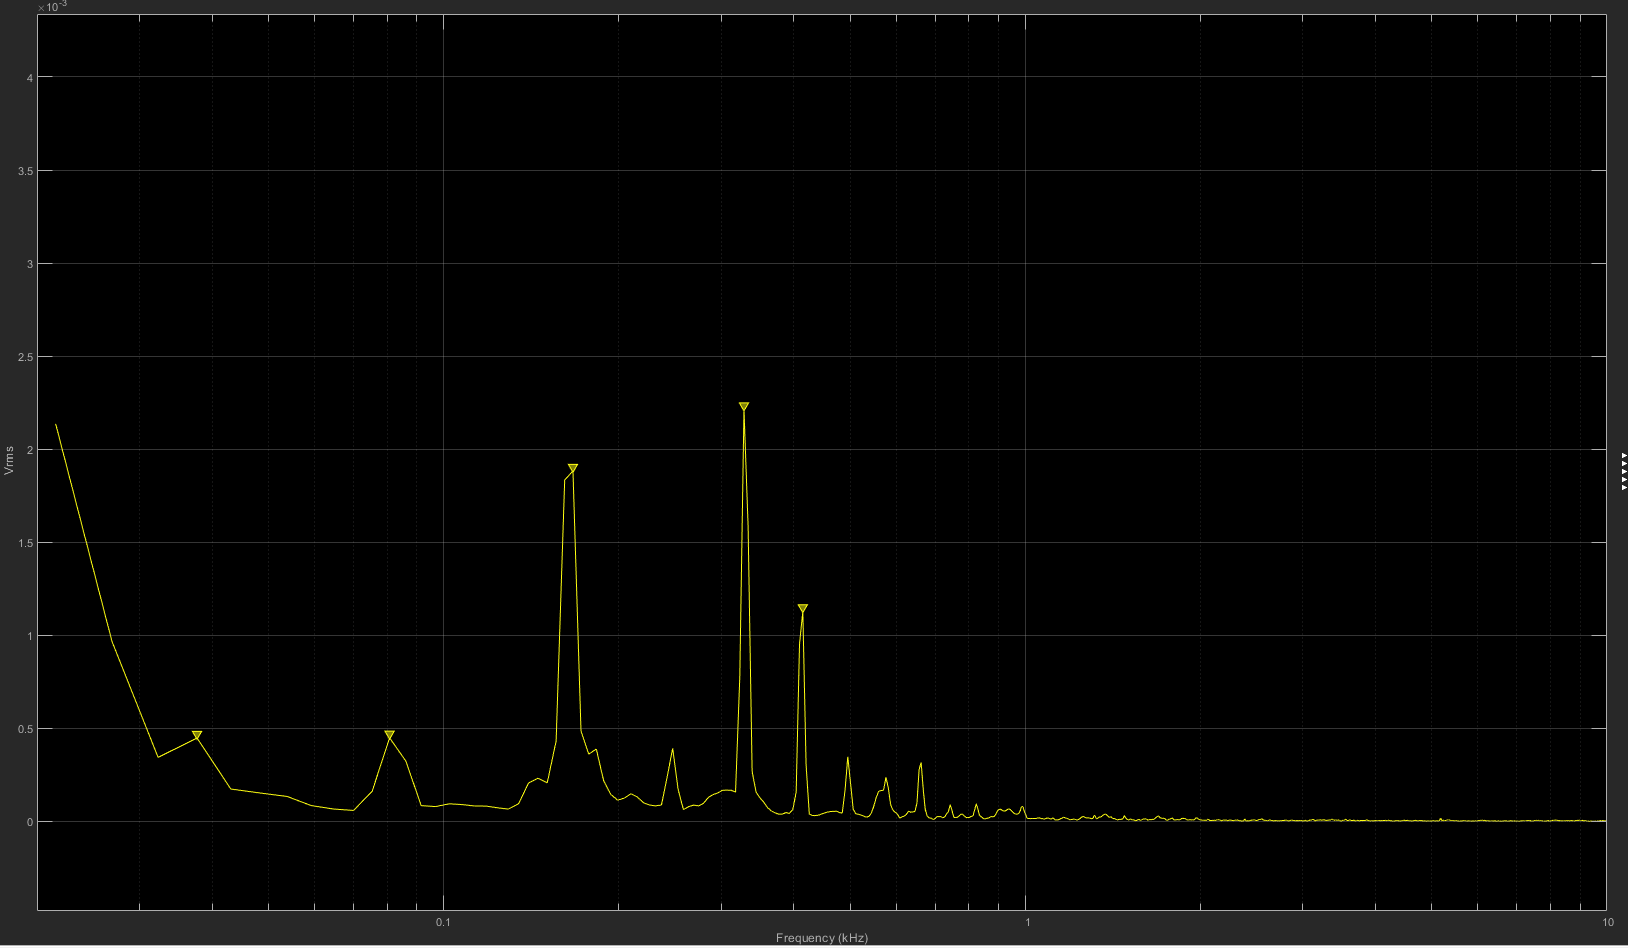
\includegraphics[scale=0.3]{resources/Epm.png}
            \caption{Amplitude vs Frequency for the palm muted low E string}
        \end{figure}
        \begin{figure}[H]\label{Eopen}
            \centering
            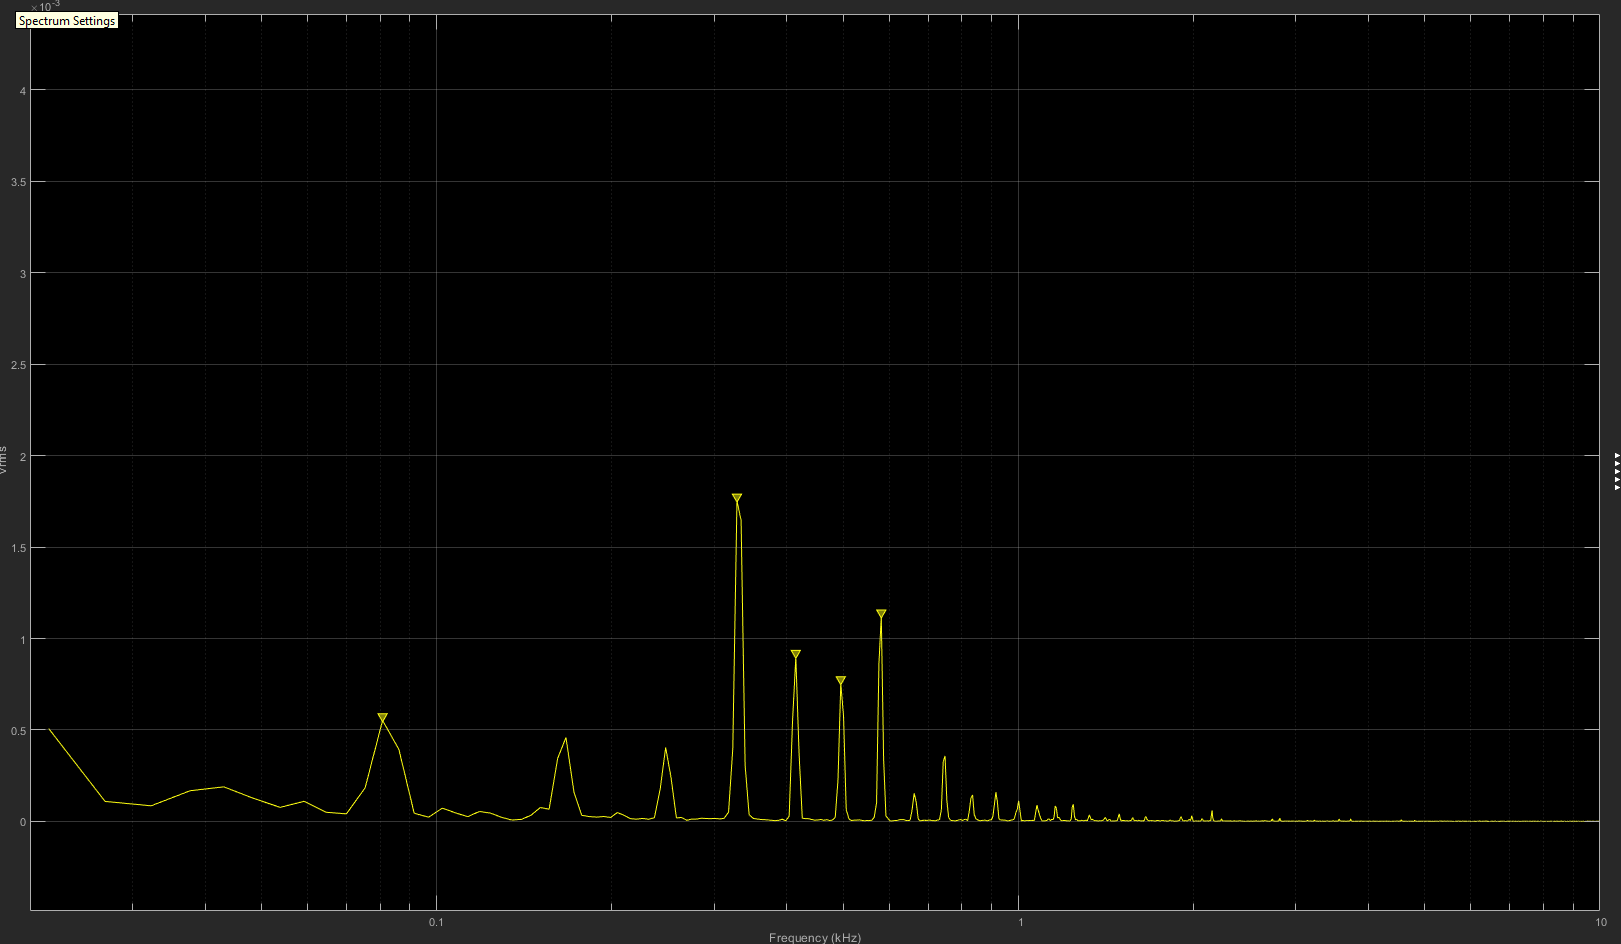
\includegraphics[scale=0.3]{resources/Eopen.png}
            \caption{Amplitude vs Frequency for the open low E string}
        \end{figure}
        
        
        \bibliography{theBib}


\end{document}